\documentclass{article}
\usepackage[utf8]{inputenc}
\usepackage[T1]{fontenc}
\usepackage{tikz}
\usepackage{amssymb}

% Blank symbol and start marker definitions
\newcommand{\blank}{\square}
\newcommand{\lmarker}{\langle}

\usetikzlibrary{automata, positioning, arrows, shapes, calc}

\begin{document}

\begin{center}
% Title
\textbf{Decider TM for $L = \{ w \in \{a,b\}^* \mid n_a(w) = n_b(w) \}$}
\vspace{1cm}

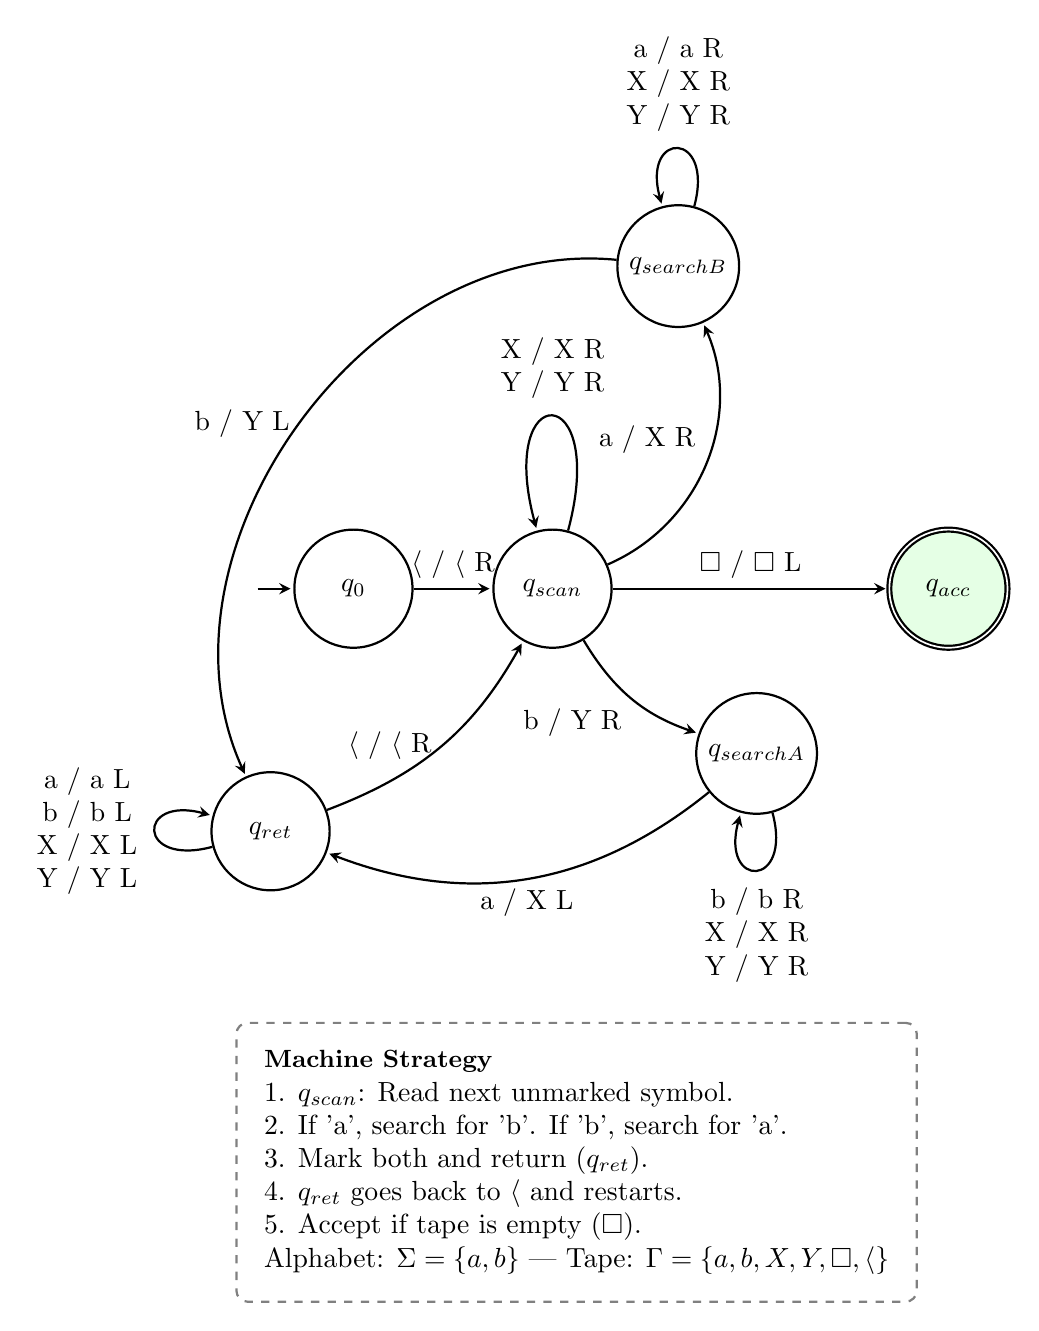
\begin{tikzpicture}[
    ->,                 
    >=stealth,          
    shorten >=1pt,      
    auto,               
    node distance=4.5cm,  % Large base distance
    thick,              
    every edge quotes/.style={font=\footnotesize, align=center}, 
    state/.style={circle, draw, minimum size=1.5cm, thick, fill=white}, 
    accept/.style={double, circle, draw, minimum size=1.5cm, thick, fill=green!10},
    initial text=       
  ]

  % --- STATE POSITIONING (SPACIOUS LAYOUT) ---
  
  \node[state, initial] (q0) {$q_{0}$};
  
  % Scanner state away from start
  \node[state, right=1cm of q0] (qscan) {$q_{scan}$};
  
  % Accept state far right
  \node[accept, right=3.5cm of qscan] (qacc) {$q_{acc}$};
  
  % --- Search states ---
  % Using large X and Y coordinates to place states in corners
  \node[state, above right=3cm and 0.5cm of qscan] (qsearchB) {$q_{searchB}$};
  \node[state, below right=1cm and 1.5cm of qscan] (qsearchA) {$q_{searchA}$};
  
  % --- Rewind state ---
  \node[state, below left=2cm and 2.5cm of qscan] (qret) {$q_{ret}$};


  % --- TRANSITIONS ---

  % 1. Initialization
  \path (q0) edge node[above] {$\lmarker$ / $\lmarker$ R} (qscan);

  % 2. Scanner
  \path (qscan) 
    % Loop
    edge[loop above, min distance=2cm, in=105, out=75] 
        node[above=1mm, align=center] {X / X R \\ Y / Y R} (qscan)
    
    % Go search for B
    edge[bend right=45] node[above left] {a / X R} (qsearchB)
    
    % Go search for A
    edge[bend right=20] node[below left] {b / Y R} (qsearchA)
    
    % Accept
    edge node[above] {$\blank$ / $\blank$ L} (qacc);

  % 3. Search for B
  \path (qsearchB) 
    % Loop
    edge[loop above, min distance=1cm, in=105, out=75] 
        node[above=1mm, align=center] {a / a R \\ X / X R \\ Y / Y R} (qsearchB)
    
    % Long return to rewind state
    edge[bend right=60] node[left, pos=0.5, align=center] {b / Y L} (qret);

  % 4. Search for A
  \path (qsearchA) 
    % Loop
    edge[loop below, min distance=1cm, in=255, out=285] 
        node[below=1mm, align=center] {b / b R \\ X / X R \\ Y / Y R} (qsearchA)
    
    % Long return to rewind state
    edge[bend left=30] node[below, pos=0.5, align=center] {a / X L} (qret);

  % 5. Rewind
  \path (qret) 
    % Loop
    edge[loop left, min distance=1cm, in=165, out=195] 
        node[left=1mm, align=center] {a / a L \\ b / b L \\ X / X L \\ Y / Y L} (qret)
        
    % Return to scan
    edge[bend right=20] node[left] {$\lmarker$ / $\lmarker$ R} (qscan);

  % --- LEGEND ---
  \node[draw=black!50, dashed, rounded corners, inner sep=10pt, align=left, anchor=north west] 
  at (-1.5, -5.5) {
    \small
    \textbf{Machine Strategy}\\
    1. $q_{scan}$: Read next unmarked symbol.\\
    2. If 'a', search for 'b'. If 'b', search for 'a'.\\
    3. Mark both and return ($q_{ret}$).\\
    4. $q_{ret}$ goes back to $\langle$ and restarts.\\
    5. Accept if tape is empty ($\blank$).\\
    Alphabet: $\Sigma = \{a, b\}$ | Tape: $\Gamma = \{a, b, X, Y, \blank, \langle\}$
  };

\end{tikzpicture}
\end{center}

\end{document}
